% !TEX TS-program = XeLaTeX
% !TEX encoding = UTF-8 Unicode

%%%%%%%%%%%%%%%%%%%%%%%%%%%%%%%%%%%%%%%%%%%%%%%%%%%%%%%%%%%%%%%%%%%%%% 
% 
%	大连理工大学博士论文 XeLaTeX 模版 —— 主文件 main.tex
% 版本:0.82
% 最后更新:2012.05.09
% 修改者:Yuri (E-mail: yuri_1985@163.com)
% 修订者:whufanwei(E-mail: dutfanwei@qq.com)
% 编译环境1:Ubuntu 12.04 + TeXLive 2011 + Emacs
% 编译环境2:Windows 7 + CTeX v2.9.2.164 + WinEdit
% 
%%%%%%%%%%%%%%%%%%%%%%%%%%%%%%%%%%%%%%%%%%%%%%%%%%%%%%%%%%%%%%%%%%%%%% 

\documentclass[12pt, a4paper, openany, twoside]{book}
%http://www.latex-community.org/forum/viewtopic.php?f=45&t=9323
%rotation of the images in latex

% 字体配置文件
% !TEX TS-program = XeLaTeX
% !TEX encoding = UTF-8 Unicode

%%%%%%%%%%%%%%%%%%%%%%%%%%%%%%%%%%%%%%%%%%%%%%%%%%%%%%%%%%%%%%%%%%%%%% 
% 
% 大连理工大学硕士论文 XeLaTeX 模版 —— 字体配置文件 fonts.tex
% 版本:0.82
% 最后更新:2012.05.08
% 修改者:Yuri (E-mail: yuri_1985@163.com)
% 修订者:whufanwei(E-mail: dutfanwei@qq.com) 
% 编译环境1:Ubuntu 12.04 + TeXLive 2011 + Emacs
% 编译环境2:Windows 7 + CTeX v2.9.2.164 + WinEdit
% 
%%%%%%%%%%%%%%%%%%%%%%%%%%%%%%%%%%%%%%%%%%%%%%%%%%%%%%%%%%%%%%%%%%%%%% 

% 英文字体设置特别推荐方案(Windows,需要安装 Adobe 字体),现代
\usepackage{fontspec}
\usepackage{xltxtra,xunicode}
\usepackage[CJKnumber,CJKchecksingle,BoldFont]{xeCJK}
\usepackage{amsmath}
\usepackage{amssymb}
\setmainfont[Mapping=tex-text]{Times New Roman}
\setsansfont[Mapping=tex-text]{Arial} 
\setmonofont{Consolas}


% 英文字体设置方案一(Windows,需要安装 LM10 字体),和 LaTeX 默认字体保持一致,经典
% \usepackage{amssymb}
% \usepackage{fontspec}
% \usepackage{amsmath}
% \usepackage[CJKnumber,CJKaddspaces,CJKchecksingle,BoldFont]{xeCJK}
% \usepackage{mathrsfs}   % 一种常用于定义泛函算子的花体字母,只有大写。
% \usepackage{bm}         % 处理数学公式中的黑斜体的宏包
% \setmainfont{LMRoman10-Regular}
% \setsansfont{LMSans10-Regular}
% \setmonofont{LMMono10-Regular}

% 英文字体设置方案二(Linux,使用自带 LM10 字体),和 LaTeX 默认字体保持一致,经典
% \usepackage{fontspec}
% \usepackage{amsmath,amssymb}
% \usepackage[CJKnumber,CJKaddspaces,CJKchecksingle,BoldFont]{xeCJK}
% \usepackage{mathrsfs}   % 一种常用于定义泛函算子的花体字母,只有大写。
% \usepackage{bm}         % 处理数学公式中的黑斜体的宏包
% \setmainfont{LMRoman10}
% \setsansfont{LMSans10}
% \setmonofont{LMMono10}

% 英文字体设置方案三(Linux,使用自带 Nimbus 字体),和 Word 模版字体保持一致,经典
% \usepackage{fontspec}
% \usepackage{mathptmx}
% \usepackage{amsmath,amssymb}
% \usepackage[CJKnumber,CJKaddspaces,CJKchecksingle,BoldFont]{xeCJK}
% \usepackage{mathrsfs}   % 一种常用于定义泛函算子的花体字母,只有大写。
% \usepackage{bm}         % 处理数学公式中的黑斜体的宏包
% \setmainfont{Nimbus Roman No9 L}
% \setsansfont{Nimbus Sans L}
% \setmonofont{Nimbus Mono L}

% 中文字体设置,使用的是 Adobe 字体,保证了在 Adobe Reader / Acrobat 下优秀的显示效果
\setCJKmainfont[BoldFont={Adobe Heiti Std},ItalicFont={Adobe Kaiti Std}]{Adobe Song Std}
\setCJKsansfont{Adobe Heiti Std}
\setCJKmonofont{Adobe Fangsong Std}

% 定义字体名称,可在此添加自定义的字体
\setCJKfamilyfont{song}{Adobe Song Std}
\setCJKfamilyfont{hei}{Adobe Heiti Std}
\setCJKfamilyfont{kai}{Adobe Kaiti Std}
\setCJKfamilyfont{fs}{Adobe Fangsong Std}
%\setCJKfamilyfont{xkai}{STXingkai}

% 自动调整中英文之间的空白
% \punctstyle{quanjiao}
\XeTeXlinebreaklocale "zh"      %中文断行
\XeTeXlinebreakskip = 0pt plus 1pt %1pt左右弹性间距
% 其他字体宏包


% 宏包配置文件
%\input{setup/packages}
%%%%%%%%%%%%%%%%%%%%%%%%%%%%%%%%%%%%%%%%%%%%%%%%%%%%%%%%%%%%%%%%%%%%%%%%%%%%%%%%
%
%   Doctoral Dissertation of Dalian University of Technology
%   By Jie Li and Ahmedin Mohammed Ahmed on the work of Hui Wang
%   package.tex
%   Version: 0.1
%   Update: 2014-04-16
%   Environment: Windows 8.1 + CTeX 2.9.2.164 + WinEdt 7.0
%   欢迎使用,如有任何意见和建议请发送邮件至 yuri_1985@163.com,感谢您的支持!
%
%%%%%%%%%%%%%%%%%%%%%%%%%%%%%%%%%%%%%%%%%%%%%%%%%%%%%%%%%%%%%%%%%%%%%%%%%%%%%%%%

% 版面控制
\usepackage[body={16.1true cm,22.0true cm}]{geometry}   %论文版芯161mm×220mm(不包括页眉页脚)
\usepackage{indentfirst}    % 首行缩进宏包
\usepackage[sf]{titlesec}   % 控制标题的宏包
\usepackage{titletoc}       % 控制目录的宏包
\renewcommand\bibname{References}
\usepackage{fancyhdr}       % 自定义页眉页脚
\usepackage{fancyref}       % 引用链接属性
\usepackage{cite}           % 支持引用的宏包
\usepackage[perpage,symbol]{footmisc}   % 脚注控制
\usepackage{layouts}        % 打印当前页面格式的宏包
\usepackage{paralist}       % 一种换行不缩进的列表格式,用 asparaenum 或者 inparaenum 环境
\usepackage[numbers]{natbib}         % 参考文献
\usepackage{fancyvrb}       % 原样输出
%\usepackage{listings}   % 粘贴源代码
%\usepackage[shortlabels]{enumitem}
% 字体
\usepackage{CJK}        % 中文支持宏包
\usepackage{amsmath}    % AMS 宏包,包含一些常用的数学字体和符号,
\usepackage{amssymb}    % 如果你引用一些不常见的字体宏包可能会与此发生冲突,请考虑略去。
\usepackage[mathscr]{eucal} % to replace the following commented package
%\usepackage{mathrsfs}   % 一种常用于定义泛函算子的花体字母,只有大写。
\usepackage[amsmath,thmmarks,hyperref]{ntheorem} % 定理类环境宏包,其中 amsmath 选项用来兼容 AMS的宏包
\usepackage{type1cm}    % 控制字体的大小
\usepackage{bm}         % 处理数学公式中的黑斜体的宏包
%\usepackage{fourier}    % 一种和Times类似的字体
\usepackage{txfonts}   % 如果你希望和 Word 的默认值保持一致,请使用此宏包
\usepackage{helvet}
\newcommand{\BigO}[1]{\ensuremath{\operatorname{O}\bigl(#1\bigr)}}
\usepackage[table]{xcolor}
\newcommand{\me}{\mathrm{e}}

\usepackage[T1]{fontenc}
\usepackage{makecell}
\renewcommand{\rothead}[3][90]{\makebox[9mm][c]{\rotatebox{#1}{\makecell[c]{#2}}}}%
\usepackage{multirow}
\usepackage{rotating,tabularx}

% 图形
\usepackage{graphicx}   % 这里引用 graphicx 宏包时没有图形驱动选项,所以请在引用图片时务必给出后缀名
\usepackage{subfigure}  % 插入子图形
\usepackage{color}      % 支持彩色
\usepackage[below]{placeins}    % 浮动图形控制宏包
\usepackage{picinpar}   % 图文混排用宏包
%\usepackage{floatflt}  % 图文混排用宏包
\usepackage{rotating}   % 图形和表格的控制
\usepackage[subfigure]{ccaption}    % 浮动图形和表格标题样式,支持插图表格的双语标题
\usepackage{setspace}   % 定制表格和图形的多行标题行距!!
\usepackage[ruled,vlined]{algorithm2e}
\usepackage[font={small}]{caption}

% 其他
\usepackage{calc}   % 在 tex 文件中具有一些计算功能,主要用在页面控制。
\usepackage{ccmap}      % 使pdfLatex生成的文件支持复制等
\usepackage[pdftex,
            CJKbookmarks=true,
            bookmarksnumbered=true,
            bookmarksopen=true,
            colorlinks=true,
            citecolor=black,
            linkcolor=black,
            anchorcolor=green,
            urlcolor=magenta,
            breaklinks=true
            ]{hyperref} % 生成有书签和超链接的 pdf















% 格式文件
%%%%%%%%%%%%%%%%%%%%%%%%%%%%%%%%%%%%%%%%%%%%%%%%%%%%%%%%%%%%%%%%%%%%%%%%%%%%%%%%%
%
%   Doctoral Dissertation of Dalian University of Technology
%   By Jie Li and Ahmedin Mohammed Ahmed on the work of Hui Wang
%   format.tex
%   Version: 0.1
%   Update: 2014-04-16
%   Environment: Windows 8.1 + CTeX 2.9.2.164 + WinEdt 7.0
%   欢迎使用,如有任何意见和建议请发送邮件至 yuri_1985@163.com,感谢您的支持!
%
%%%%%%%%%%%%%%%%%%%%%%%%%%%%%%%%%%%%%%%%%%%%%%%%%%%%%%%%%%%%%%%%%%%%%%%%%%%%%%%%

%%%%%%%%%%%%%%%%%%%%%%%%%%%%%%%%%%%%%%%%%%%%%%%%%%%%%%%%%%%%%%%%%%%%%%%%%%%%%%%%80
% Settings of Pages
% 页面设置
%%%%%%%%%%%%%%%%%%%%%%%%%%%%%%%%%%%%%%%%%%%%%%%%%%%%%%%%%%%%%%%%%%%%%%%%%%%%%%%%80
% A4 纸张
\setlength{\paperwidth}{21.0cm}
\setlength{\paperheight}{29.7cm}

% Size of the content
% 设置正文尺寸大小
\setlength{\textwidth}{16.0cm}
\setlength{\textheight}{23.7cm}

% To make the content in the middle of the page
% 设置正文区在正中间
\newlength \mymargin
\setlength{\mymargin}{(\paperwidth-\textwidth)/2}
\setlength{\oddsidemargin}{(\mymargin)-1in}
\setlength{\evensidemargin}{(\mymargin)-1in}


% 设置正文区偏移量,奇数页向右偏,偶数页向左偏
\newlength \myshift
\setlength{\myshift}{0.35cm}     % 双面打印的奇偶页偏移值,可根据需要修改,建议小于 0.5 cm。
\addtolength{\oddsidemargin}{\myshift}
\addtolength{\evensidemargin}{-\myshift}
\setlength{\topmargin}{-0.75cm}
\setlength{\headheight}{0.50cm}
\setlength{\headsep}{0.90cm}
\setlength{\footskip}{1.47cm}

% Adjustment of equations
% 公式的精调
\allowdisplaybreaks[4]  % 可以让公式在排不下的时候分页排,这可避免页面有大段空白。

%下面这组命令使浮动对象的缺省值稍微宽松一点,从而防止幅度
%对象占据过多的文本页面,也可以防止在很大空白的浮动页上放置
%很小的图形。
\renewcommand{\textfraction}{0.15}
\renewcommand{\topfraction}{0.85}
\renewcommand{\bottomfraction}{0.65}
\renewcommand{\floatpagefraction}{0.60}

%%%%%%%%%%%%%%%%%%%%%%%%%%%%%%%%%%%%%%%%%%%%%%%%%%%%%%%%%%%%%%%%%%%%%%%%%%%%%%%%80
% Font and Size
% 字体字号定义
%%%%%%%%%%%%%%%%%%%%%%%%%%%%%%%%%%%%%%%%%%%%%%%%%%%%%%%%%%%%%%%%%%%%%%%%%%%%%%%%80
% Indent of Chinese
% 中文段落缩进和 ~ 字符替换
%\CJKindent                              % 首行缩进两个汉字
%\sloppy
%\CJKspace                              % 中英文混排的断行
\%CJKtilde                               % 重新定义~,用~隔开中英文

% Chinese Font
% 中文字体
\newcommand{\song}{\CJKfamily{song}}    % 宋体 (Font of SONG)
\newcommand{\fs}{\CJKfamily{fs}}        % 仿宋 (Font of FANG SONG)
\newcommand{\kai}{\CJKfamily{kai}}      % 楷体
\newcommand{\hei}{\CJKfamily{hei}}      % 黑体
%\newcommand{\li}{\CJKfamily{li}}        % 隶书
%\newcommand{\you}{\CJKfamily{you}}      % 幼圆
%\newcommand{\xk}{\CJKfamily{STXingkai}}
% 字号

\newcommand{\yihao}{\fontsize{26pt}{39pt}\selectfont}               % 一号,1.5 倍行距
%\newcommand{\twentysix}{\fontsize{26pt}{39pt}\selectfont}               % 一号,1.5 倍行距
\newcommand{\xiaoyi}{\fontsize{24pt}{30pt}\selectfont}              % 小一,1.25倍行距
%\newcommand{\twentyfour}{\fontsize{24pt}{30pt}\selectfont}              % 小一,1.25倍行距
%\newcommand{\erhao}{\fontsize{22pt}{27.5pt}\selectfont}             % 二号,1.25倍行距
\newcommand{\xiaoer}{\fontsize{18pt}{22.5pt}\selectfont}            % 小二,1.25倍行距
\newcommand{\eighteen}{\fontsize{18pt}{27pt}\selectfont}            % 18 pt and 27 pt line space
\newcommand{\sanhao}{\fontsize{16pt}{20pt}\selectfont}              % 三号,1.25倍行距
\newcommand{\xiaosan}{\fontsize{15pt}{18.75pt}\selectfont}          % 小三,1.25倍行距
\newcommand{\daxiaosi}{\fontsize{12pt}{18pt}\selectfont}            % 小四,1.5 倍行距
\newcommand{\ltwelve}{\fontsize{12pt}{18pt}\selectfont}             % large twelve with 12pt, 18pt line space
\newcommand{\sihao}{\fontsize{14pt}{17pt}\selectfont}               % 四号,1.25倍行距
\newcommand{\fourteen}{\fontsize{14pt}{17pt}\selectfont}            % 14 pt and 17 pt line space
\newcommand{\thirteen}{\fontsize{13pt}{19.5pt}\selectfont}          % 13 pt, 19.5 pt line space
\newcommand{\xiaosi}{\fontsize{12pt}{15pt}\selectfont}              % 小四,1.25倍行距
\newcommand{\twelve}{\fontsize{12pt}{15pt}\selectfont}              % 小四(12 pt),1.25倍行距
\newcommand{\eleven}{\fontsize{11pt}{13.75pt}\selectfont}           % 11 pt, 13.75 line space
\newcommand{\dawu}{\fontsize{10.5pt}{18pt}\selectfont}              % 五号,1.75倍行距
\newcommand{\zhongwu}{\fontsize{10.5pt}{15pt}\selectfont}           % 五号,1.5 倍行距
\newcommand{\wuhao}{\fontsize{10.5pt}{10.5pt}\selectfont}           % 五号,单倍行距
\newcommand{\ten}{\fontsize{10pt}{10pt}\selectfont}                 % 五号,单倍行距
\newcommand{\xiaowu}{\fontsize{9pt}{9pt}\selectfont}                % 小五,单倍行距

% defaultfont 默认字体命令
\def\defaultfont{\renewcommand{\baselinestretch}{1.25}
\fontsize{12pt}{15pt}\selectfont}

% Font in Table of Content
% 设置目录字体和行间距
\def\defaultmenufont{\renewcommand{\baselinestretch}{1.22}
\fontsize{12pt}{12pt}}

% Content with fixed distance and underline
% 固定距离内容填入及下划线
\makeatletter
    \newcommand\fixeddistanceleft[2][1cm]{{\hb@xt@ #1{#2\hss}}}
    \newcommand\fixeddistancecenter[2][1cm]{{\hb@xt@ #1{\hss#2\hss}}}
    \newcommand\fixeddistanceright[2][1cm]{{\hb@xt@ #1{\hss#2}}}
    \newcommand\fixedunderlineleft[2][1cm]{\underline{\hb@xt@ #1{#2\hss}}}
    \newcommand\fixedunderlinecenter[2][1cm]{\underline{\hb@xt@ #1{\hss#2\hss}}}
    \newcommand\fixedunderlineright[2][1cm]{\underline{\hb@xt@ #1{\hss#2}}}
\makeatother
%%%%%%%%%%%%%%%%%%%%%%%%%%%%%%%%%%%%%%%%%%%%%%%%%%%%%%%%%%%%%%%%%%%%%%%%%%%%%%%%80
% Subtitles
% 标题相关
%%%%%%%%%%%%%%%%%%%%%%%%%%%%%%%%%%%%%%%%%%%%%%%%%%%%%%%%%%%%%%%%%%%%%%%%%%%%%%%%80
% Definition, Theorem, etc
% 定义、定理等环境
%\theoremstyle{plain}
%\theoremheaderfont{\hei\bf}
%\theorembodyfont{\song\rmfamily}
%\newtheorem{definition}{\hei 定义}[chapter]
%\newtheorem{example}{\hei 例}[chapter]
%\newtheorem{algorithm}{\hei 算法}[chapter]
%\newtheorem{theorem}{\hei 定理}[chapter]
%\newtheorem{axiom}{\hei 公理}[chapter]
%\newtheorem{proposition}[theorem]{\hei 命题}
%\newtheorem{property}{\hei 性质}
%\newtheorem{lemma}[theorem]{\hei 引理}
%\newtheorem{corollary}{\hei 推论}[chapter]
%\newtheorem{remark}{\hei 注解}[chapter]
%\newenvironment{proof}{{\hei证明 }}%
%{\hfill $\square$ \vskip 4mm}
%\theoremsymbol{$\square$}
%%%%%%%%%%%%%%%%%%%%%%%%%%%%%%%%%%%%%%%%%%%%%%%%%%%%%%%%%%
\theoremstyle{plain}
\theoremheaderfont{}
\theorembodyfont{}
\newtheorem{definition}{}[chapter]
\newtheorem{example}{}[chapter]
%\newtheorem{algorithm}{}[chapter]
\newtheorem{theorem}{}[chapter]
\newtheorem{axiom}{}[chapter]
\newtheorem{proposition}[theorem]{}
\newtheorem{property}{}
\newtheorem{lemma}[theorem]{}
\newtheorem{corollary}{}[chapter]
\newtheorem{remark}{}[chapter]
\newenvironment{proof}{}%
{\hfill $\square$ \vskip 4mm}
%\theoremsymbol{$\square$}


% 目录标题
\renewcommand\contentsname{\hfill 中文目录 \hfill}
%\renewcommand\listfigurename{\hfill 图~表~目~录 \hfill} %王辉修改
%\renewcommand\listtablename{\hfill 表~格~目~录 \hfill} %王辉修改
%\renewcommand{\bibname}{\hfill 参~考~文~献 \hfill}
%\renewcommand{\algorithmcfname}{算法}
%\renewcommand{\algorithmcfname}{Algorithm}

%%%%%%%%%%%%%%%%%%%%%%%%%%%%%%%%%%%%%%%%%%%%%%%%%%%%%%%%%%%%%%%%%%%%%%%%%%%%%%%%80
% Chapters, sections
% 段落章节
%%%%%%%%%%%%%%%%%%%%%%%%%%%%%%%%%%%%%%%%%%%%%%%%%%%%%%%%%%%%%%%%%%%%%%%%%%%%%%%%80
\setcounter{secnumdepth}{4}
\setcounter{tocdepth}{4}
% 设置章、节、小节、小小节的间距
\titleformat{\chapter}[hang]{\eighteen}{\eighteen\thechapter}{10pt}{\eighteen}
\titlespacing{\chapter}{0pt}{-3ex  plus .1ex minus .2ex}{3.3ex}
\titleformat{\section}[hang]{\fourteen}{\fourteen\thesection}{0.5em}{}{}
\titlespacing{\section}{0pt}{0.5em}{0.5em}
\titleformat{\subsection}[hang]{\twelve}{\twelve\thesubsection}{0.5em}{}{}
\titlespacing{\subsection}{0pt}{0.5em}{0.3em}
\titleformat{\subsubsection}[hang]{}{\thesubsubsection}{0.5em}{}{}
\titlespacing{\subsubsection}{0pt}{0.3em}{0pt}
% 缩小目录中各级标题之间的缩进
\dottedcontents{chapter}[0.32cm]{\vspace{0.2em}}{1.0em}{5pt}
\dottedcontents{section}[1.32cm]{}{1.8em}{5pt}
\dottedcontents{subsection}[2.32cm]{}{2.7em}{5pt}
\dottedcontents{subsubsection}[3.32cm]{}{3.4em}{5pt}

%
% 段落之间的竖直距离
\setlength{\parskip}{1.2pt}
% Line space
% 定义行距
\renewcommand{\baselinestretch}{1.27}
% Line space of references
% 参考文献条目间行间距
\setlength{\bibsep}{1pt}

%%%%%%%%%%%%%%%%%%%%%%%%%%%%%%%%%%%%%%%%%%%%%%%%%%%%%%%%%%%%%%%%%%%%%%%%%%%%%%%%80
% Head and foot, using package of fancyhdr
% 页眉和页脚 使用 fancyhdr 宏包
%%%%%%%%%%%%%%%%%%%%%%%%%%%%%%%%%%%%%%%%%%%%%%%%%%%%%%%%%%%%%%%%%%%%%%%%%%%%%%%%80

\newcommand{\makeheadrule}{%
    \makebox[0pt][l]{\rule[.7\baselineskip]{\headwidth}{0.5pt}}%
    \vskip-.8\baselineskip}

\makeatletter
\renewcommand{\headrule}{%
    {\if@fancyplain\let\headrulewidth\plainheadrulewidth\fi
     \makeheadrule}}

\pagestyle{fancyplain}

\fancyhf{}
\fancyhead[CO]{\ten Dalian University of Technology Doctoral Dissertation}
\fancyhead[CE]{\ten\@etitle}
\fancyfoot[C,C]{\ten--~\thepage~--}

% Clear Header Style on the Last Empty Odd pages
\makeatletter
\def\cleardoublepage{\clearpage\if@twoside \ifodd\c@page\else%
    \hbox{}%
    \thispagestyle{empty}%              % Empty header styles
    \newpage%
    \if@twocolumn\hbox{}\newpage\fi\fi\fi}



%%%%%%%%%%%%%%%%%%%%%%%%%%%%%%%%%%%%%%%%%%%%%%%%%%%%%%%%%%%%%%%%%%%%%%%%%%%%%%%%80
% 调整列表环境的垂直间距
%%%%%%%%%%%%%%%%%%%%%%%%%%%%%%%%%%%%%%%%%%%%%%%%%%%%%%%%%%%%%%%%%%%%%%%%%%%%%%%%80
\let\orig@Itemize =\itemize
\let\orig@Enumerate =\enumerate
\let\orig@Description =\description

\def\Myspacing{\itemsep=1ex \topsep=-4ex \partopsep=-2ex \parskip=-1ex \parsep=2ex}
\def\newitemsep{
\renewenvironment{itemize}{\orig@Itemize\Myspacing}{\endlist}
\renewenvironment{enumerate}{\orig@Enumerate\Myspacing}{\endlist}
\renewenvironment{description}{\orig@Description\Myspacing}{\endlist}
}
\def\olditemsep{
\renewenvironment{itemize}{\orig@Itemize}{\endlist}
\renewenvironment{enumerate}{\orig@Enumerate}{\endlist}
\renewenvironment{description}{\orig@Description}{\endlist}
}
\renewcommand{\labelenumi}{(\arabic{enumi})}
\newitemsep

% fancyvrb宏包中\VerbatimInput的格式设置
\fvset{fontsize=\small, frame=single, baselinestretch=1}

% 修改引用的格式
\newcommand{\ucite}[1]{$^{\mbox{\scriptsize \citep{#1}}}$} % 增加 \ucite 命令使显示的引用为上标形式
\newcommand{\citeup}[1]{$^{\mbox{\scriptsize \citep{#1}}}$} % for WinEdt users

%参考文献
%\addtolength{\bibsep}{-0.2cm}

%%%%%%%%%%%%%%%%%%%%%%%%%%%%%%%%%%%%%%%%%%%%%%%%%%%%%%%%%%%%%%%%%%%%%%%%%%%%%%%%80
% Figures and tables
% 图形表格
%%%%%%%%%%%%%%%%%%%%%%%%%%%%%%%%%%%%%%%%%%%%%%%%%%%%%%%%%%%%%%%%%%%%%%%%%%%%%%%%80

\renewcommand{\figurename}{Fig.}
\renewcommand{\tablename}{Tab.}
%\captionstyle{\centering}
%\hangcaption
\captiondelim{\hspace{1em}}
%\captionnamefont{\song\rmfamily\zhongwu\selectfont}
%\captiontitlefont{\song\rmfamily\zhongwu\selectfont}

\newcommand{\tablepage}[2]{\begin{minipage}{#1}\vspace{0.5ex} #2 \vspace{0.5ex}\end{minipage}}
\newcommand{\returnpage}[2]{\begin{minipage}{#1}\vspace{0.5ex} #2 \vspace{-1.5ex}\end{minipage}}


%%%%%%%%%%%%%%%%%%%%%%%%%%%%%%%%%%%%%%%%%%%%%%%%%%%%%%%%%%%%%%%%%%%%%%%%%%%%%%%%80
% 定义题头格言的格式
%%%%%%%%%%%%%%%%%%%%%%%%%%%%%%%%%%%%%%%%%%%%%%%%%%%%%%%%%%%%%%%%%%%%%%%%%%%%%%%%80

%\newsavebox{\AphorismAuthor}
%\newenvironment{Aphorism}[1]
%{\vspace{0.5cm}\begin{sloppypar} \slshape
%\sbox{\AphorismAuthor}{#1}
%\begin{quote}\small\itshape }
%{\\ \hspace*{\fill}------\hspace{0.2cm} \usebox{\AphorismAuthor}
%\end{quote}
%\end{sloppypar}\vspace{0.5cm}}

%自定义一个空命令,用于注释掉文本中不需要的部分。
\newcommand{\comment}[1]{}

% This is the flag for longer version
\newcommand{\longer}[2]{#1}

\newcommand{\ds}{\displaystyle}

% define graph scale
\def\gs{1.0}

%%%%%%%%%%%%%%%%%%%%%%%%%%%%%%%%%%%%%%%%%%%%%%%%%%%%%%%%%%%%%%%%%%%%%%%%%%%%%%%%80
% 自定义项目列表标签及格式 \begin{denselist} 列表项 \end{denselist}
%%%%%%%%%%%%%%%%%%%%%%%%%%%%%%%%%%%%%%%%%%%%%%%%%%%%%%%%%%%%%%%%%%%%%%%%%%%%%%%%80
\newcounter{newlist} %自定义新计数器
\newenvironment{denselist}[1][temp]{%%%%%定义新环境:可改变的列表题目
\begin{list}{\textbf{#1} (\arabic{newlist})} %%标签格式
    {
    \usecounter{newlist}
     \setlength{\labelwidth}{22pt} %标签盒子宽度
     \setlength{\labelsep}{0cm} %标签与列表文本距离
     \setlength{\leftmargin}{0cm} %左右边界
     \setlength{\rightmargin}{0cm}
     \setlength{\parsep}{0ex} %段落间距
     \setlength{\itemsep}{0ex} %标签间距
     \setlength{\itemindent}{44pt} %标签缩进量
     \setlength{\listparindent}{44pt} %段落缩进量
    }}
{\end{list}}%%%%%

%%%%%%%%%%%%%%%%%%%%%%%%%%%%%%%%%%%%%%%%%%%%%%%%%%%%%%%%%%%%%%%%%%%%%%%%%%%%%%%%80
% cover
% 封面摘要
%%%%%%%%%%%%%%%%%%%%%%%%%%%%%%%%%%%%%%%%%%%%%%%%%%%%%%%%%%%%%%%%%%%%%%%%%%%%%%%%80
%\def\cdegree#1{\def\@cdegree{#1}}\def\@cdegree{}
\def\ctitle#1{\def\@ctitle{#1}}\def\@ctitle{}
%\def\etitle#1{\def\@etitle{#1}}\def\@etitle{}
\def\department#1{\def\@department{#1}}\def\@department{}
\def\caffil#1{\def\@caffil{#1}}\def\@caffil{}
\def\csubject#1{\def\@csubject{#1}}\def\@csubject{}
\def\cauthor#1{\def\@cauthor{#1}}\def\@cauthor{}
\def\cauthorno#1{\def\@cauthorno{#1}}\def\@cauthorno{}
\def\csupervisor#1{\def\@csupervisor{#1}}\def\@csupervisor{}
\def\cdate#1{\def\@cdate{#1}}\def\@cdate{}
\long\def\cabstract#1{\long\def\@cabstract{#1}}\long\def\@cabstract{}
\def\ckeywords#1{\def\@ckeywords{#1}}\def\@ckeywords{}
\def\etitle#1{\def\@etitle{#1}}\def\@etitle{}
\long\def\eabstract#1{\long\def\@eabstract{#1}}\long\def\@eabstract{}
\def\ekeywords#1{\def\@ekeywords{#1}}\def\@ekeywords{}



\def\eoriginality{
    \renewcommand{\baselinestretch}{1.61}
    % Originality Declaration
    \newpage
    \thispagestyle{empty}
    \begin{center}
    \eighteen {Dalian University of Technology Dissertation \\ Originality Declaration}
    \end{center}
    \parbox[t][7.68cm][c]{\textwidth}{\twelve
            \noindent
             I declare that this dissertation is the result of an independent research I have made under the supervision of my supervisor. It does not contain any published or unpublished works or research results by other individuals or institutions apart from those that have been referenced in the form of references or notes. All individuals and institutions that have made contributions to my research have been acknowledged in the Acknowledgement.

           \noindent
           % \vspace{0.47cm}
            I am fully aware that I myself will bear all the legal responsibility arising from violation of the above declaration. \\
            ~~~~~~\\
        }
        \noindent

        {\twelve Dissertation Title: \fixedunderlinecenter[12.6cm]{\@etitle}}\\
        ~~\\

        {\twelve Author Signature: \fixeddistanceleft[12.6cm]{\underline{\hspace{7.3cm}}\hfill Date: \underline{\hspace{1.1cm}}/{\underline{\hspace{1.6cm}}/{\underline{\hspace{1.1cm}}}}}}\\

    \renewcommand{\baselinestretch}{1.27}
    \cleardoublepage
}

\def\originality{
    \renewcommand{\baselinestretch}{1.61}
    % 独创性说明
    \newpage
    \thispagestyle{empty}
    \begin{center}
        \parbox[t][1.52cm][c]{\textwidth}{{\xiaoer\song\centerline{大连理工大学学位论文独创性声明}}}
        \parbox[t][7.68cm][c]{\textwidth}{\sihao\fs
            \noindent
            作者郑重声明:所呈交的学位论文,是本人在导师的指导下进行研究工作所取得的成果。%
            尽我所知,除文中已经注明引用内容和致谢的地方外,%
            本论文不包含其他个人或集体已经发表的研究成果,%
            也不包含其他已申请学位或其他用途使用过的成果。%
            与我一同工作的同志对本研究所做的贡献均已在论文中做了明确的说明并表示了谢意。%

            \noindent
            \vspace{0.47cm}
            若有不实之处,本人愿意承担相关法律责任。
        }
        \noindent
        %\parbox[t][0.58cm][c]{\textwidth}
        {\sihao\fs 学{\hfill}位{\hfill}论{\hfill}文{\hfill}题{\hfill}目{\hfill}:\fixedunderlinecenter[12.6cm]{\@ctitle}}\\
        \sihao\fs~~~\\
        %\parbox[t][1.22cm][c]{\textwidth}
        {\sihao\fs 作{\hfill}者{\hfill}签{\hfill}名{\hfill}:\fixeddistanceleft[12.6cm]{\underline{\hspace{5.8cm}}\hfill
	       日期:\underline{\hspace{1.4cm}}~年~{\underline{\hspace{0.7cm}}~月~{\underline{\hspace{0.7cm}}~日~}}}}\\
    \end{center}
    \renewcommand{\baselinestretch}{1.27}

    \cleardoublepage
}

\def\makecover{
    \begin{titlepage}
    % Cover
        \newpage
        \thispagestyle{empty}
            \begin{center}
            \parbox[t][3cm][c]{12.8cm}
            {
                \begin{center}
                    {\eighteen {\@etitle}\\}
                    {\eighteen{\textit{\@ctitle}}\\}
                    %{\eighteen{( \textit{\@ctitle})}\\}
                \end{center}
            }
            \parbox[c][16.8cm][c]{\textwidth}
            {

                \begin{center}

                    {~~\\
                    \twelve{by} \\
                    ~~~\\
                    }
                    {\defaultfont {\@cauthor}\\}
                    {\defaultfont(\textit{\@cauthorno})\\}
                    {~~\\
                    \twelve {to} \\
                    ~~~\\
                    }
                    {\twelve {\textit{\@department}}\\}
                    {~~~\\
                    \defaultfont {in partial fulfillment of the requirements}\\
                    \defaultfont {for the degree of}\\
                    \defaultfont {Doctor of Philosophy}\\
                    \defaultfont {in the subject of}\\
                    }
                    {\defaultfont {\textit{\@csubject}}\\}
                    {~~~\\
                    \defaultfont {on}\\}
                    {\defaultfont {\textit{\@cdate}}\\}
                    {~~\\
                    \defaultfont {Dissertation Supervisor}\\
                    ~~~\\}
                    {\defaultfont{\textit{\@csupervisor}}\\}
                    {~~\\
                    ~~\\
                    ~~~\\}
                    %\end{tabular}
                \end{center}

            }

            {
                \begin{figure}[h]
                    \centering
                    
\includegraphics[scale=1]{DUT.pdf}
                \end{figure}
                \vspace{-0.35cm}
                \defaultfont{Dalian University of Technology}
            }
            \end{center}
        \cleardoublepage
    \end{titlepage}
}

\def\eauthorization
{
\newpage
\begin{center}
    \eighteen Dalian University of Technology Doctoral Dissertation Copyright Use Authorization
\end{center}

\twelve
I fully understand relevant regulations regarding university dissertation copyright. Copyright of theses at university during PhD period belongs to Dalian University of Technology, allowing theses to be consulted and borrowed. University has right to retain theses and submit copies and electronic editions to national departments and institutions concerned. University can index relevant database for retrieval using part or the whole of this dissertation. University can photocopy, print in reduced format or scan to keep and compile this dissertation.
\\

\noindent
Dissertation Title: \fixedunderlinecenter[12.6cm]{\@etitle}\\
~~\\
Author's Signature: \fixeddistanceleft[12.6cm]{\underline{\hspace{7.3cm}}\hfill
    Date: \underline{\hspace{1.1cm}}/{\underline{\hspace{1.6cm}}/{\underline{\hspace{1.1cm}}}}}\\
    ~~~\\
Supervisor's Signature: \fixeddistanceleft[12.0cm]{\underline{\hspace{6.7cm}}\hfill
	 Date: \underline{\hspace{1.1cm}}/{\underline{\hspace{1.6cm}}/{\underline{\hspace{1.1cm}}}}}\\
\renewcommand{\baselinestretch}{1.27}
}

\def\authorization
{
\newpage
\begin{center}
    \eighteen\song~大连理工大学学位论文版权使用授权书~
\end{center}

\sihao\fs\noindent
  本人完全了解学校有关学位论文知识产权的规定,%
在校攻读学位期间论文工作的知识产权属于大连理工大学,允许论文被查阅和借阅。%
学校有权保留论文并向国家有关部门或机构送交论文的复印件和电子版,%
可以将本学位论文的全部或部分内容编入有关数据库进行检索,%
可以采用影印、缩印、或扫描等复制手段保存和汇编本学位论文。%
\\

\noindent
学{\hfill}位{\hfill}论{\hfill}文{\hfill}题{\hfill}目{\hfill}:\fixedunderlinecenter[12.6cm]{\@ctitle}\\
作{\hfill}者{\hfill}签{\hfill}名{\hfill}:\fixeddistanceleft[12.6cm]{\underline{\hspace{6.0cm}}\hfill
    ~~日期:\underline{\hspace{1.4cm}}~年~{\underline{\hspace{0.7cm}}~月~{\underline{\hspace{0.7cm}}~日~}}}\\
导{\hfill}师{\hfill}签{\hfill}名{\hfill}:\fixeddistanceleft[12.6cm]{\underline{\hspace{6.0cm}}\hfill
	 ~~日期:\underline{\hspace{1.4cm}}~年~{\underline{\hspace{0.7cm}}~月~{\underline{\hspace{0.7cm}}~日~}}}\\
\renewcommand{\baselinestretch}{1.27}
}

\def\makeabstract{
    \defaultfont

    \chapter*{\hfill Abstract \hfill}
    %\addcontentsline{toe}{chapter}{Abstract}
    \setcounter{page}{1}
    \@eabstract
    \vspace{0.53cm}

    {\textbf{Keywords:} \@ekeywords}

    \defaultfont
    \cleardoublepage
    \chapter*{}
    \vspace{-1.38cm}
    \vspace{-0.36cm}
    \begin{center}
    {
       \eighteen\song{摘~~~~~~~~要}\\
    }
    \end{center}
    \vspace{0.11cm}

    \@cabstract

    \vspace{0.53cm}

    {\hei{关键词:{\fs\@ckeywords}}}

    \defaultfont
    \cleardoublepage
}

\makeatletter
\def\hlinewd#1{%
  \noalign{\ifnum0=`}\fi\hrule \@height #1 \futurelet
   \reserved@a\@xhline}
\makeatother

%定义索引生成
\def\generateindex
{
    \addcontentsline{toc}{chapter}{\indexname}
    \printindex
    \cleardoublepage
}

\raggedbottom

% 格式文件结束

%%%%%%%%%%%%%%%%%%%%%%%%%%%%%%%%%%%%%%%%%%%%%%%%%%%%%%%%%%%%%%%%%%%%%%%%%%%%%%%%
%
%   Doctoral Dissertation of Dalian University of Technology
%   By Jie Li and Ahmedin Mohammed Ahmed on the work of Hui Wang
%   format.tex
%   Version: 0.1
%   Update: 2014-04-16
%   Environment: Windows 8.1 + CTeX 2.9.2.164 + WinEdt 7.0
%   欢迎使用,如有任何意见和建议请发送邮件至 yuri_1985@163.com,感谢您的支持!
%
%%%%%%%%%%%%%%%%%%%%%%%%%%%%%%%%%%%%%%%%%%%%%%%%%%%%%%%%%%%%%%%%%%%%%%%%%%%%%%%%

%%%%%%%%%%%%%%%%%%%%%%%%%%%%%%%%%%%%%%%%%%%%%%%%%%%%%%%%%%%%%%%%%%%%%%%%%%%%%%%%80
% Settings of Pages
% 页面设置
%%%%%%%%%%%%%%%%%%%%%%%%%%%%%%%%%%%%%%%%%%%%%%%%%%%%%%%%%%%%%%%%%%%%%%%%%%%%%%%%80
% A4 纸张
\setlength{\paperwidth}{21.0cm}
\setlength{\paperheight}{29.7cm}

% Size of the content
% 设置正文尺寸大小
\setlength{\textwidth}{16.0cm}
\setlength{\textheight}{23.7cm}

% To make the content in the middle of the page
% 设置正文区在正中间
\newlength \mymargin
\setlength{\mymargin}{(\paperwidth-\textwidth)/2}
\setlength{\oddsidemargin}{(\mymargin)-1in}
\setlength{\evensidemargin}{(\mymargin)-1in}


% 设置正文区偏移量,奇数页向右偏,偶数页向左偏
\newlength \myshift
\setlength{\myshift}{0.35cm}     % 双面打印的奇偶页偏移值,可根据需要修改,建议小于 0.5 cm。
\addtolength{\oddsidemargin}{\myshift}
\addtolength{\evensidemargin}{-\myshift}
\setlength{\topmargin}{-0.75cm}
\setlength{\headheight}{0.50cm}
\setlength{\headsep}{0.90cm}
\setlength{\footskip}{1.47cm}

% Adjustment of equations
% 公式的精调
\allowdisplaybreaks[4]  % 可以让公式在排不下的时候分页排,这可避免页面有大段空白。

%下面这组命令使浮动对象的缺省值稍微宽松一点,从而防止幅度
%对象占据过多的文本页面,也可以防止在很大空白的浮动页上放置
%很小的图形。
\renewcommand{\textfraction}{0.15}
\renewcommand{\topfraction}{0.85}
\renewcommand{\bottomfraction}{0.65}
\renewcommand{\floatpagefraction}{0.60}

%%%%%%%%%%%%%%%%%%%%%%%%%%%%%%%%%%%%%%%%%%%%%%%%%%%%%%%%%%%%%%%%%%%%%%%%%%%%%%%%80
% Font and Size
% 字体字号定义
%%%%%%%%%%%%%%%%%%%%%%%%%%%%%%%%%%%%%%%%%%%%%%%%%%%%%%%%%%%%%%%%%%%%%%%%%%%%%%%%80
% Indent of Chinese
% 中文段落缩进和 ~ 字符替换
%\CJKindent                              % 首行缩进两个汉字
%\sloppy
%\CJKspace                              % 中英文混排的断行
\%CJKtilde                               % 重新定义~,用~隔开中英文

% Chinese Font
% 中文字体
\newcommand{\song}{\CJKfamily{song}}    % 宋体 (Font of SONG)
\newcommand{\fs}{\CJKfamily{fs}}        % 仿宋 (Font of FANG SONG)
\newcommand{\kai}{\CJKfamily{kai}}      % 楷体
\newcommand{\hei}{\CJKfamily{hei}}      % 黑体
%\newcommand{\li}{\CJKfamily{li}}        % 隶书
%\newcommand{\you}{\CJKfamily{you}}      % 幼圆
%\newcommand{\xk}{\CJKfamily{STXingkai}}
% 字号

\newcommand{\yihao}{\fontsize{26pt}{39pt}\selectfont}               % 一号,1.5 倍行距
%\newcommand{\twentysix}{\fontsize{26pt}{39pt}\selectfont}               % 一号,1.5 倍行距
\newcommand{\xiaoyi}{\fontsize{24pt}{30pt}\selectfont}              % 小一,1.25倍行距
%\newcommand{\twentyfour}{\fontsize{24pt}{30pt}\selectfont}              % 小一,1.25倍行距
%\newcommand{\erhao}{\fontsize{22pt}{27.5pt}\selectfont}             % 二号,1.25倍行距
\newcommand{\xiaoer}{\fontsize{18pt}{22.5pt}\selectfont}            % 小二,1.25倍行距
\newcommand{\eighteen}{\fontsize{18pt}{27pt}\selectfont}            % 18 pt and 27 pt line space
\newcommand{\sanhao}{\fontsize{16pt}{20pt}\selectfont}              % 三号,1.25倍行距
\newcommand{\xiaosan}{\fontsize{15pt}{18.75pt}\selectfont}          % 小三,1.25倍行距
\newcommand{\daxiaosi}{\fontsize{12pt}{18pt}\selectfont}            % 小四,1.5 倍行距
\newcommand{\ltwelve}{\fontsize{12pt}{18pt}\selectfont}             % large twelve with 12pt, 18pt line space
\newcommand{\sihao}{\fontsize{14pt}{17pt}\selectfont}               % 四号,1.25倍行距
\newcommand{\fourteen}{\fontsize{14pt}{17pt}\selectfont}            % 14 pt and 17 pt line space
\newcommand{\thirteen}{\fontsize{13pt}{19.5pt}\selectfont}          % 13 pt, 19.5 pt line space
\newcommand{\xiaosi}{\fontsize{12pt}{15pt}\selectfont}              % 小四,1.25倍行距
\newcommand{\twelve}{\fontsize{12pt}{15pt}\selectfont}              % 小四(12 pt),1.25倍行距
\newcommand{\eleven}{\fontsize{11pt}{13.75pt}\selectfont}           % 11 pt, 13.75 line space
\newcommand{\dawu}{\fontsize{10.5pt}{18pt}\selectfont}              % 五号,1.75倍行距
\newcommand{\zhongwu}{\fontsize{10.5pt}{15pt}\selectfont}           % 五号,1.5 倍行距
\newcommand{\wuhao}{\fontsize{10.5pt}{10.5pt}\selectfont}           % 五号,单倍行距
\newcommand{\ten}{\fontsize{10pt}{10pt}\selectfont}                 % 五号,单倍行距
\newcommand{\xiaowu}{\fontsize{9pt}{9pt}\selectfont}                % 小五,单倍行距

% defaultfont 默认字体命令
\def\defaultfont{\renewcommand{\baselinestretch}{1.25}
\fontsize{12pt}{15pt}\selectfont}

% Font in Table of Content
% 设置目录字体和行间距
\def\defaultmenufont{\renewcommand{\baselinestretch}{1.22}
\fontsize{12pt}{12pt}}

% Content with fixed distance and underline
% 固定距离内容填入及下划线
\makeatletter
    \newcommand\fixeddistanceleft[2][1cm]{{\hb@xt@ #1{#2\hss}}}
    \newcommand\fixeddistancecenter[2][1cm]{{\hb@xt@ #1{\hss#2\hss}}}
    \newcommand\fixeddistanceright[2][1cm]{{\hb@xt@ #1{\hss#2}}}
    \newcommand\fixedunderlineleft[2][1cm]{\underline{\hb@xt@ #1{#2\hss}}}
    \newcommand\fixedunderlinecenter[2][1cm]{\underline{\hb@xt@ #1{\hss#2\hss}}}
    \newcommand\fixedunderlineright[2][1cm]{\underline{\hb@xt@ #1{\hss#2}}}
\makeatother
%%%%%%%%%%%%%%%%%%%%%%%%%%%%%%%%%%%%%%%%%%%%%%%%%%%%%%%%%%%%%%%%%%%%%%%%%%%%%%%%80
% Subtitles
% 标题相关
%%%%%%%%%%%%%%%%%%%%%%%%%%%%%%%%%%%%%%%%%%%%%%%%%%%%%%%%%%%%%%%%%%%%%%%%%%%%%%%%80
% Definition, Theorem, etc
% 定义、定理等环境
%\theoremstyle{plain}
%\theoremheaderfont{\hei\bf}
%\theorembodyfont{\song\rmfamily}
%\newtheorem{definition}{\hei 定义}[chapter]
%\newtheorem{example}{\hei 例}[chapter]
%\newtheorem{algorithm}{\hei 算法}[chapter]
%\newtheorem{theorem}{\hei 定理}[chapter]
%\newtheorem{axiom}{\hei 公理}[chapter]
%\newtheorem{proposition}[theorem]{\hei 命题}
%\newtheorem{property}{\hei 性质}
%\newtheorem{lemma}[theorem]{\hei 引理}
%\newtheorem{corollary}{\hei 推论}[chapter]
%\newtheorem{remark}{\hei 注解}[chapter]
%\newenvironment{proof}{{\hei证明 }}%
%{\hfill $\square$ \vskip 4mm}
%\theoremsymbol{$\square$}
%%%%%%%%%%%%%%%%%%%%%%%%%%%%%%%%%%%%%%%%%%%%%%%%%%%%%%%%%%
\theoremstyle{plain}
\theoremheaderfont{}
\theorembodyfont{}
\newtheorem{definition}{}[chapter]
\newtheorem{example}{}[chapter]
%\newtheorem{algorithm}{}[chapter]
\newtheorem{theorem}{}[chapter]
\newtheorem{axiom}{}[chapter]
\newtheorem{proposition}[theorem]{}
\newtheorem{property}{}
\newtheorem{lemma}[theorem]{}
\newtheorem{corollary}{}[chapter]
\newtheorem{remark}{}[chapter]
\newenvironment{proof}{}%
{\hfill $\square$ \vskip 4mm}
%\theoremsymbol{$\square$}


% 目录标题
\renewcommand\contentsname{\hfill 中文目录 \hfill}
%\renewcommand\listfigurename{\hfill 图~表~目~录 \hfill} %王辉修改
%\renewcommand\listtablename{\hfill 表~格~目~录 \hfill} %王辉修改
%\renewcommand{\bibname}{\hfill 参~考~文~献 \hfill}
%\renewcommand{\algorithmcfname}{算法}
%\renewcommand{\algorithmcfname}{Algorithm}

%%%%%%%%%%%%%%%%%%%%%%%%%%%%%%%%%%%%%%%%%%%%%%%%%%%%%%%%%%%%%%%%%%%%%%%%%%%%%%%%80
% Chapters, sections
% 段落章节
%%%%%%%%%%%%%%%%%%%%%%%%%%%%%%%%%%%%%%%%%%%%%%%%%%%%%%%%%%%%%%%%%%%%%%%%%%%%%%%%80
\setcounter{secnumdepth}{4}
\setcounter{tocdepth}{4}
% 设置章、节、小节、小小节的间距
\titleformat{\chapter}[hang]{\eighteen}{\eighteen\thechapter}{10pt}{\eighteen}
\titlespacing{\chapter}{0pt}{-3ex  plus .1ex minus .2ex}{3.3ex}
\titleformat{\section}[hang]{\fourteen}{\fourteen\thesection}{0.5em}{}{}
\titlespacing{\section}{0pt}{0.5em}{0.5em}
\titleformat{\subsection}[hang]{\twelve}{\twelve\thesubsection}{0.5em}{}{}
\titlespacing{\subsection}{0pt}{0.5em}{0.3em}
\titleformat{\subsubsection}[hang]{}{\thesubsubsection}{0.5em}{}{}
\titlespacing{\subsubsection}{0pt}{0.3em}{0pt}
% 缩小目录中各级标题之间的缩进
\dottedcontents{chapter}[0.32cm]{\vspace{0.2em}}{1.0em}{5pt}
\dottedcontents{section}[1.32cm]{}{1.8em}{5pt}
\dottedcontents{subsection}[2.32cm]{}{2.7em}{5pt}
\dottedcontents{subsubsection}[3.32cm]{}{3.4em}{5pt}

%
% 段落之间的竖直距离
\setlength{\parskip}{1.2pt}
% Line space
% 定义行距
\renewcommand{\baselinestretch}{1.27}
% Line space of references
% 参考文献条目间行间距
\setlength{\bibsep}{1pt}

%%%%%%%%%%%%%%%%%%%%%%%%%%%%%%%%%%%%%%%%%%%%%%%%%%%%%%%%%%%%%%%%%%%%%%%%%%%%%%%%80
% Head and foot, using package of fancyhdr
% 页眉和页脚 使用 fancyhdr 宏包
%%%%%%%%%%%%%%%%%%%%%%%%%%%%%%%%%%%%%%%%%%%%%%%%%%%%%%%%%%%%%%%%%%%%%%%%%%%%%%%%80

\newcommand{\makeheadrule}{%
    \makebox[0pt][l]{\rule[.7\baselineskip]{\headwidth}{0.5pt}}%
    \vskip-.8\baselineskip}

\makeatletter
\renewcommand{\headrule}{%
    {\if@fancyplain\let\headrulewidth\plainheadrulewidth\fi
     \makeheadrule}}

\pagestyle{fancyplain}

\fancyhf{}
\fancyhead[CO]{\ten Dalian University of Technology Doctoral Dissertation}
\fancyhead[CE]{\ten\@etitle}
\fancyfoot[C,C]{\ten--~\thepage~--}

% Clear Header Style on the Last Empty Odd pages
\makeatletter
\def\cleardoublepage{\clearpage\if@twoside \ifodd\c@page\else%
    \hbox{}%
    \thispagestyle{empty}%              % Empty header styles
    \newpage%
    \if@twocolumn\hbox{}\newpage\fi\fi\fi}



%%%%%%%%%%%%%%%%%%%%%%%%%%%%%%%%%%%%%%%%%%%%%%%%%%%%%%%%%%%%%%%%%%%%%%%%%%%%%%%%80
% 调整列表环境的垂直间距
%%%%%%%%%%%%%%%%%%%%%%%%%%%%%%%%%%%%%%%%%%%%%%%%%%%%%%%%%%%%%%%%%%%%%%%%%%%%%%%%80
\let\orig@Itemize =\itemize
\let\orig@Enumerate =\enumerate
\let\orig@Description =\description

\def\Myspacing{\itemsep=1ex \topsep=-4ex \partopsep=-2ex \parskip=-1ex \parsep=2ex}
\def\newitemsep{
\renewenvironment{itemize}{\orig@Itemize\Myspacing}{\endlist}
\renewenvironment{enumerate}{\orig@Enumerate\Myspacing}{\endlist}
\renewenvironment{description}{\orig@Description\Myspacing}{\endlist}
}
\def\olditemsep{
\renewenvironment{itemize}{\orig@Itemize}{\endlist}
\renewenvironment{enumerate}{\orig@Enumerate}{\endlist}
\renewenvironment{description}{\orig@Description}{\endlist}
}
\renewcommand{\labelenumi}{(\arabic{enumi})}
\newitemsep

% fancyvrb宏包中\VerbatimInput的格式设置
\fvset{fontsize=\small, frame=single, baselinestretch=1}

% 修改引用的格式
\newcommand{\ucite}[1]{$^{\mbox{\scriptsize \citep{#1}}}$} % 增加 \ucite 命令使显示的引用为上标形式
\newcommand{\citeup}[1]{$^{\mbox{\scriptsize \citep{#1}}}$} % for WinEdt users

%参考文献
%\addtolength{\bibsep}{-0.2cm}

%%%%%%%%%%%%%%%%%%%%%%%%%%%%%%%%%%%%%%%%%%%%%%%%%%%%%%%%%%%%%%%%%%%%%%%%%%%%%%%%80
% Figures and tables
% 图形表格
%%%%%%%%%%%%%%%%%%%%%%%%%%%%%%%%%%%%%%%%%%%%%%%%%%%%%%%%%%%%%%%%%%%%%%%%%%%%%%%%80

\renewcommand{\figurename}{Fig.}
\renewcommand{\tablename}{Tab.}
%\captionstyle{\centering}
%\hangcaption
\captiondelim{\hspace{1em}}
%\captionnamefont{\song\rmfamily\zhongwu\selectfont}
%\captiontitlefont{\song\rmfamily\zhongwu\selectfont}

\newcommand{\tablepage}[2]{\begin{minipage}{#1}\vspace{0.5ex} #2 \vspace{0.5ex}\end{minipage}}
\newcommand{\returnpage}[2]{\begin{minipage}{#1}\vspace{0.5ex} #2 \vspace{-1.5ex}\end{minipage}}


%%%%%%%%%%%%%%%%%%%%%%%%%%%%%%%%%%%%%%%%%%%%%%%%%%%%%%%%%%%%%%%%%%%%%%%%%%%%%%%%80
% 定义题头格言的格式
%%%%%%%%%%%%%%%%%%%%%%%%%%%%%%%%%%%%%%%%%%%%%%%%%%%%%%%%%%%%%%%%%%%%%%%%%%%%%%%%80

%\newsavebox{\AphorismAuthor}
%\newenvironment{Aphorism}[1]
%{\vspace{0.5cm}\begin{sloppypar} \slshape
%\sbox{\AphorismAuthor}{#1}
%\begin{quote}\small\itshape }
%{\\ \hspace*{\fill}------\hspace{0.2cm} \usebox{\AphorismAuthor}
%\end{quote}
%\end{sloppypar}\vspace{0.5cm}}

%自定义一个空命令,用于注释掉文本中不需要的部分。
\newcommand{\comment}[1]{}

% This is the flag for longer version
\newcommand{\longer}[2]{#1}

\newcommand{\ds}{\displaystyle}

% define graph scale
\def\gs{1.0}

%%%%%%%%%%%%%%%%%%%%%%%%%%%%%%%%%%%%%%%%%%%%%%%%%%%%%%%%%%%%%%%%%%%%%%%%%%%%%%%%80
% 自定义项目列表标签及格式 \begin{denselist} 列表项 \end{denselist}
%%%%%%%%%%%%%%%%%%%%%%%%%%%%%%%%%%%%%%%%%%%%%%%%%%%%%%%%%%%%%%%%%%%%%%%%%%%%%%%%80
\newcounter{newlist} %自定义新计数器
\newenvironment{denselist}[1][temp]{%%%%%定义新环境:可改变的列表题目
\begin{list}{\textbf{#1} (\arabic{newlist})} %%标签格式
    {
    \usecounter{newlist}
     \setlength{\labelwidth}{22pt} %标签盒子宽度
     \setlength{\labelsep}{0cm} %标签与列表文本距离
     \setlength{\leftmargin}{0cm} %左右边界
     \setlength{\rightmargin}{0cm}
     \setlength{\parsep}{0ex} %段落间距
     \setlength{\itemsep}{0ex} %标签间距
     \setlength{\itemindent}{44pt} %标签缩进量
     \setlength{\listparindent}{44pt} %段落缩进量
    }}
{\end{list}}%%%%%

%%%%%%%%%%%%%%%%%%%%%%%%%%%%%%%%%%%%%%%%%%%%%%%%%%%%%%%%%%%%%%%%%%%%%%%%%%%%%%%%80
% cover
% 封面摘要
%%%%%%%%%%%%%%%%%%%%%%%%%%%%%%%%%%%%%%%%%%%%%%%%%%%%%%%%%%%%%%%%%%%%%%%%%%%%%%%%80
%\def\cdegree#1{\def\@cdegree{#1}}\def\@cdegree{}
\def\ctitle#1{\def\@ctitle{#1}}\def\@ctitle{}
%\def\etitle#1{\def\@etitle{#1}}\def\@etitle{}
\def\department#1{\def\@department{#1}}\def\@department{}
\def\caffil#1{\def\@caffil{#1}}\def\@caffil{}
\def\csubject#1{\def\@csubject{#1}}\def\@csubject{}
\def\cauthor#1{\def\@cauthor{#1}}\def\@cauthor{}
\def\cauthorno#1{\def\@cauthorno{#1}}\def\@cauthorno{}
\def\csupervisor#1{\def\@csupervisor{#1}}\def\@csupervisor{}
\def\cdate#1{\def\@cdate{#1}}\def\@cdate{}
\long\def\cabstract#1{\long\def\@cabstract{#1}}\long\def\@cabstract{}
\def\ckeywords#1{\def\@ckeywords{#1}}\def\@ckeywords{}
\def\etitle#1{\def\@etitle{#1}}\def\@etitle{}
\long\def\eabstract#1{\long\def\@eabstract{#1}}\long\def\@eabstract{}
\def\ekeywords#1{\def\@ekeywords{#1}}\def\@ekeywords{}



\def\eoriginality{
    \renewcommand{\baselinestretch}{1.61}
    % Originality Declaration
    \newpage
    \thispagestyle{empty}
    \begin{center}
    \eighteen {Dalian University of Technology Dissertation \\ Originality Declaration}
    \end{center}
    \parbox[t][7.68cm][c]{\textwidth}{\twelve
            \noindent
             I declare that this dissertation is the result of an independent research I have made under the supervision of my supervisor. It does not contain any published or unpublished works or research results by other individuals or institutions apart from those that have been referenced in the form of references or notes. All individuals and institutions that have made contributions to my research have been acknowledged in the Acknowledgement.

           \noindent
           % \vspace{0.47cm}
            I am fully aware that I myself will bear all the legal responsibility arising from violation of the above declaration. \\
            ~~~~~~\\
        }
        \noindent

        {\twelve Dissertation Title: \fixedunderlinecenter[12.6cm]{\@etitle}}\\
        ~~\\

        {\twelve Author Signature: \fixeddistanceleft[12.6cm]{\underline{\hspace{7.3cm}}\hfill Date: \underline{\hspace{1.1cm}}/{\underline{\hspace{1.6cm}}/{\underline{\hspace{1.1cm}}}}}}\\

    \renewcommand{\baselinestretch}{1.27}
    \cleardoublepage
}

\def\originality{
    \renewcommand{\baselinestretch}{1.61}
    % 独创性说明
    \newpage
    \thispagestyle{empty}
    \begin{center}
        \parbox[t][1.52cm][c]{\textwidth}{{\xiaoer\song\centerline{大连理工大学学位论文独创性声明}}}
        \parbox[t][7.68cm][c]{\textwidth}{\sihao\fs
            \noindent
            作者郑重声明:所呈交的学位论文,是本人在导师的指导下进行研究工作所取得的成果。%
            尽我所知,除文中已经注明引用内容和致谢的地方外,%
            本论文不包含其他个人或集体已经发表的研究成果,%
            也不包含其他已申请学位或其他用途使用过的成果。%
            与我一同工作的同志对本研究所做的贡献均已在论文中做了明确的说明并表示了谢意。%

            \noindent
            \vspace{0.47cm}
            若有不实之处,本人愿意承担相关法律责任。
        }
        \noindent
        %\parbox[t][0.58cm][c]{\textwidth}
        {\sihao\fs 学{\hfill}位{\hfill}论{\hfill}文{\hfill}题{\hfill}目{\hfill}:\fixedunderlinecenter[12.6cm]{\@ctitle}}\\
        \sihao\fs~~~\\
        %\parbox[t][1.22cm][c]{\textwidth}
        {\sihao\fs 作{\hfill}者{\hfill}签{\hfill}名{\hfill}:\fixeddistanceleft[12.6cm]{\underline{\hspace{5.8cm}}\hfill
	       日期:\underline{\hspace{1.4cm}}~年~{\underline{\hspace{0.7cm}}~月~{\underline{\hspace{0.7cm}}~日~}}}}\\
    \end{center}
    \renewcommand{\baselinestretch}{1.27}

    \cleardoublepage
}

\def\makecover{
    \begin{titlepage}
    % Cover
        \newpage
        \thispagestyle{empty}
            \begin{center}
            \parbox[t][3cm][c]{12.8cm}
            {
                \begin{center}
                    {\eighteen {\@etitle}\\}
                    {\eighteen{\textit{\@ctitle}}\\}
                    %{\eighteen{( \textit{\@ctitle})}\\}
                \end{center}
            }
            \parbox[c][16.8cm][c]{\textwidth}
            {

                \begin{center}

                    {~~\\
                    \twelve{by} \\
                    ~~~\\
                    }
                    {\defaultfont {\@cauthor}\\}
                    {\defaultfont(\textit{\@cauthorno})\\}
                    {~~\\
                    \twelve {to} \\
                    ~~~\\
                    }
                    {\twelve {\textit{\@department}}\\}
                    {~~~\\
                    \defaultfont {in partial fulfillment of the requirements}\\
                    \defaultfont {for the degree of}\\
                    \defaultfont {Doctor of Philosophy}\\
                    \defaultfont {in the subject of}\\
                    }
                    {\defaultfont {\textit{\@csubject}}\\}
                    {~~~\\
                    \defaultfont {on}\\}
                    {\defaultfont {\textit{\@cdate}}\\}
                    {~~\\
                    \defaultfont {Dissertation Supervisor}\\
                    ~~~\\}
                    {\defaultfont{\textit{\@csupervisor}}\\}
                    {~~\\
                    ~~\\
                    ~~~\\}
                    %\end{tabular}
                \end{center}

            }

            {
                \begin{figure}[h]
                    \centering
                    
\includegraphics[scale=1]{DUT.pdf}
                \end{figure}
                \vspace{-0.35cm}
                \defaultfont{Dalian University of Technology}
            }
            \end{center}
        \cleardoublepage
    \end{titlepage}
}

\def\eauthorization
{
\newpage
\begin{center}
    \eighteen Dalian University of Technology Doctoral Dissertation Copyright Use Authorization
\end{center}

\twelve
I fully understand relevant regulations regarding university dissertation copyright. Copyright of theses at university during PhD period belongs to Dalian University of Technology, allowing theses to be consulted and borrowed. University has right to retain theses and submit copies and electronic editions to national departments and institutions concerned. University can index relevant database for retrieval using part or the whole of this dissertation. University can photocopy, print in reduced format or scan to keep and compile this dissertation.
\\

\noindent
Dissertation Title: \fixedunderlinecenter[12.6cm]{\@etitle}\\
~~\\
Author's Signature: \fixeddistanceleft[12.6cm]{\underline{\hspace{7.3cm}}\hfill
    Date: \underline{\hspace{1.1cm}}/{\underline{\hspace{1.6cm}}/{\underline{\hspace{1.1cm}}}}}\\
    ~~~\\
Supervisor's Signature: \fixeddistanceleft[12.0cm]{\underline{\hspace{6.7cm}}\hfill
	 Date: \underline{\hspace{1.1cm}}/{\underline{\hspace{1.6cm}}/{\underline{\hspace{1.1cm}}}}}\\
\renewcommand{\baselinestretch}{1.27}
}

\def\authorization
{
\newpage
\begin{center}
    \eighteen\song~大连理工大学学位论文版权使用授权书~
\end{center}

\sihao\fs\noindent
  本人完全了解学校有关学位论文知识产权的规定,%
在校攻读学位期间论文工作的知识产权属于大连理工大学,允许论文被查阅和借阅。%
学校有权保留论文并向国家有关部门或机构送交论文的复印件和电子版,%
可以将本学位论文的全部或部分内容编入有关数据库进行检索,%
可以采用影印、缩印、或扫描等复制手段保存和汇编本学位论文。%
\\

\noindent
学{\hfill}位{\hfill}论{\hfill}文{\hfill}题{\hfill}目{\hfill}:\fixedunderlinecenter[12.6cm]{\@ctitle}\\
作{\hfill}者{\hfill}签{\hfill}名{\hfill}:\fixeddistanceleft[12.6cm]{\underline{\hspace{6.0cm}}\hfill
    ~~日期:\underline{\hspace{1.4cm}}~年~{\underline{\hspace{0.7cm}}~月~{\underline{\hspace{0.7cm}}~日~}}}\\
导{\hfill}师{\hfill}签{\hfill}名{\hfill}:\fixeddistanceleft[12.6cm]{\underline{\hspace{6.0cm}}\hfill
	 ~~日期:\underline{\hspace{1.4cm}}~年~{\underline{\hspace{0.7cm}}~月~{\underline{\hspace{0.7cm}}~日~}}}\\
\renewcommand{\baselinestretch}{1.27}
}

\def\makeabstract{
    \defaultfont

    \chapter*{\hfill Abstract \hfill}
    %\addcontentsline{toe}{chapter}{Abstract}
    \setcounter{page}{1}
    \@eabstract
    \vspace{0.53cm}

    {\textbf{Keywords:} \@ekeywords}

    \defaultfont
    \cleardoublepage
    \chapter*{}
    \vspace{-1.38cm}
    \vspace{-0.36cm}
    \begin{center}
    {
       \eighteen\song{摘~~~~~~~~要}\\
    }
    \end{center}
    \vspace{0.11cm}

    \@cabstract

    \vspace{0.53cm}

    {\hei{关键词:{\fs\@ckeywords}}}

    \defaultfont
    \cleardoublepage
}

\makeatletter
\def\hlinewd#1{%
  \noalign{\ifnum0=`}\fi\hrule \@height #1 \futurelet
   \reserved@a\@xhline}
\makeatother

%定义索引生成
\def\generateindex
{
    \addcontentsline{toc}{chapter}{\indexname}
    \printindex
    \cleardoublepage
}

\raggedbottom

% 格式文件结束


%以下由王辉增加(2012年12月16日),主要是修改英文目录和图标目录
%Revision 1: 目录中的点的稠密程度
\makeatletter
\def\@dotsep{0.3}%就在这儿改,把2改成其他什么,默认是4.5,就是点之间距离为4.5mu
\makeatother



%Revision 2: Formatting Table of Contents in Chinese and English
%Font
\titlecontents{chapter}[10mm]
{\fontsize{12pt}{15pt}}
{\contentslabel{4em}}
{}
{\titlerule*{.}\contentspage}
%
\titlecontents{section}[12mm]
{\fontsize{12pt}{15pt}}
{\contentslabel{2em}}
{}
{\titlerule*{.}\contentspage}
%
\titlecontents{subsection}[23mm]
{\fontsize{12pt}{15pt}}
{\contentslabel{3em}}
{}
{\titlerule*{.}\contentspage}

%Indent
\dottedcontents{chapter}[0.32cm]{\vspace{0.2em}}{1.0em}{5pt}
\dottedcontents{section}[1.32cm]{}{1.8em}{5pt}
\dottedcontents{subsection}[2.32cm]{}{2.7em}{5pt}
\dottedcontents{subsubsection}[3.32cm]{}{3.4em}{5pt}

%Revision 3: Content in English
\makeatletter
\newcommand\engcontentsname{\hfill CONTENTS \hfill}
%\newcommand\engcontentsname{CONTENTS}
\newcommand\tableofengcontents{%
    \if@twocolumn
      \@restonecoltrue\onecolumn
    \else
      \@restonecolfalse
    \fi
    \chapter*{\engcontentsname
        \@mkboth{%
           \MakeUppercase\engcontentsname}{\MakeUppercase\engcontentsname}}%
    \@starttoc{toe}% !!!!Define a new contents!!!!
    \if@restonecol\twocolumn\fi
    }
\newcommand\addengcontents[2]{%
    \addcontentsline{toe}{#1}{\protect\numberline{\csname the#1\endcsname}#2}}
\makeatother
\newcommand\echapter[1]{\addengcontents{chapter}{#1}}
\newcommand\esection[1]{\addengcontents{section}{#1}}
\newcommand\esubsection[1]{\addengcontents{subsection}{#1}}
\newcommand\esubsubsection[1]{\addengcontents{subsubsection}{#1}}




\begin{document}
% 格式文件

% 定义所有的图片文件在 figures 子目录下
\graphicspath{{figures/}}

% 前言
\frontmatter
\pagenumbering{Roman}
%%%%%%%%%%%%%%%%%%%%%%%%%%%%%%%%%%%%%%%%%%%%%%%%%%%%%%%%%%%%%%%%%%%%%%%%%%%%%%%%
%
%   Doctoral Dissertation of Dalian University of Technology
%   By Jie Li and Ahmedin Mohammed Ahmed on the work of Hui Wang
%   cover.tex
%   Version: 0.1
%   Update: 2014-04-16
%   Environment: Windows 8.1 + CTeX 2.9.2.164 + WinEdt 7.0
%   欢迎使用,如有任何意见和建议请发送邮件至 yuri_1985@163.com,感谢您的支持!
%
%%%%%%%%%%%%%%%%%%%%%%%%%%%%%%%%%%%%%%%%%%%%%%%%%%%%%%%%%%%%%%%%%%%%%%%%%%%%%%%%

\etitle{Data Management Middleware Protocols in Ad-hoc Social Networks}
\ctitle{自组织社会网络中的数据管理中间件协议}
%\ctitle{大连理工大学博士学位论文格式规范}

\cauthor{Ahmedin Mohammed Ahmed}
\cauthorno{11117019}
\department{School of Software}
\csubject{Computer Science and Technology}


\cdate{November 22, 2014}
\csupervisor{Feng Xia}

\eabstract{
Ad-hoc social networks (ASNETs) provide infrastructure-less settings for mobile users to communicate with each other opportunistically. Taking advantage of the users' social characteristics collected from modern sensor devices can enhance and fine tune the performance of mobile ad-hoc networking. Middleware design for this socially-aware paradigm is of paramount importance to develop innovative applications and services easily and efficiently. Nevertheless, due to various limitations such as lack of centralized management, device heterogeneity, unreliable wireless communication, mobility, resource constraints, or the need to support different traffic types, a number of new challenges have emerged recently.  One of the main challenges is performance degradation and implementation inefficiencies, which are caused by the gap between the application and lower layer protocols. In addition, managing data poses a severe challenge for both human beings and wireless networking systems, which usually only model protocols by ignoring or within a certain consideration of users' social and mobility information. ASNETs can be of immense use in case of pervasive conference/meeting and ubiquitous emergency situations. Most scenarios of this network clearly illustrate the relevance of incorporating important services or modules (e.g., data management) with middleware design for proper wireless network operation.

In previous works, ad-hoc networking frameworks have been proposed and data management issues were investigated in which social awareness was not considered. To address the downside, we focus on developing a formal framework for ASNETs middleware upon which design and proposal of our data management protocols can be based. We take advantages of social networks and mobile ad-hoc networks to integrate social-awareness and user mobility, respectively. This leads us to investigate various aspects of data management middleware problems including data availability, load distribution and users' cooperative participation in partitioned communities. ASNETs differ from social networks in which disconnections are the norm instead of the exception. Traditionally, different ideal approaches are widely used to facilitate data availability, even load distribution and users cooperation. However, the quality of wireless links would be affected by many factors like mobility, overhead and users' selfish behavior. A data replication methodology and community-partitioning concept is applied intensively throughout the course of this study to tackle the aforementioned challenges. To the best of our knowledge, this is the first work to explore data availability, load distribution and selfishness issues together in ASNETs.

The accessibility and availability of ASNET services can be assured by replication approaches. Replica allocation helps to avoid data losses in case of an unpredictable group mobility that causes community partition and also aids in reducing the number of hops when a data is transmitted from source to destination. However, it is impossible to replicate all data items on every node because of the limited resources. The question here is, where and how we should allocate the data replicas to gain high data accessibility and availability.  We first contribute to this line of research with replication protocol for maximizing availability of a data by proposing ComPAS, a community-partitioning aware replica allocation method. In ComPAS, we apply an efficient and consistent way to store replicas for each user's data. Consequently, we choose the numbers of replicas depending on the replication budget of the system and its desired availability. Its goal include integration of social relationship for placing copy of the data in the community to achieve better consistency by keeping the replica read cost, relocation cost and traffic as low as possible. It tries to balance the community storage space load as next goal. ComPAS offers a more interesting pattern in terms of read cost as compared to other schemes and it is highly efficient when relocation of replicas happened in the network.

ASNET systems are poised with challenges of performance degradation and poor scalability. This is typically caused by an uneven load distribution of operations and the susceptibility of link failure. The fair functionality of any distributed system can be realized by allowing its integral computational elements to work cooperatively. An effective load balancing mechanism guarantees optimal use of the system resources whereby no broker remains in an under-loaded state while any other broker is being overloaded. In many of today's distributed environments including ASNETs, users are linked with limited resources such as storage space and bandwidth that inherently inflicts tangible delays. This leads the users to rely on inter-resource communications and load exchange throughout the network. To be able to fully benefit from such networking systems, data availability and resource distribution are key services, where issues of load distribution, partitioning and fault tolerance present a common challenge. Herein, we enhance the data management performance by proposing Co-Lab, community-based event dissemination with load balancing and fairness mechanism. This protocol employs interest similarity and filter replication approaches for clustering brokers in a community. Its goals are to achieve better load distribution more uniformly among brokers and circumvent highly overloaded brokers by keeping the reliability as high as possible. Performance evaluations indicate that Co-Lab has promising advantages by achieving relatively better load balance, reduced overall load, and robustness against failures.

Another shortcoming of existing data management protocols is the assumption that users are cooperative when participating in operations such as forwarding data. If nodes refuse to collaborate in the network services, end-to-end connection may not be possible. Such unwilling (selfish) behavior can greatly degrade the network performance. Therefore, it is essential to detect such selfish users and mitigate their impact on the performance of other well-behaving users. Even though solutions for detecting selfish users have been explored before, a few fundamental shortcomings surrounding the problem have remained unaddressed, particularly in data dissemination and forwarding for ASNET services. Thus, we attempt to design an algorithm that gives each user the autonomy to identify and exclude selfish users. Features like these can often be observed in biological processes such as bacteria and inspired us for augmenting our new cooperative architectural concept to the replica allocation protocol. In this work, we propose a biologically inspired algorithm to detect and mitigate the impact of selfish users called BoDMaS that employs ComPAS as a data replication model. Using social and biological mechanisms, BoDMaS assesses and classifies users, and denies selfish user participation. The effectiveness of the proposed scheme is evaluated using different metrics selected for evaluation, demonstrating its ability of accurately detecting selfishness in replication operations for ASNET environments.
}

\ekeywords{Ad-hoc Social Networks; Middleware; Data Management; Replication; Load Balancing; Selfishness}

\cabstract{
自组织社会网络为移动用户间提供了基础设施无关的机会性沟通环境。充分利用由现代传感设备采集的用户社会性特征有助于提升和改善移动自组织网络的性能。其中,以社会感知机制为基础设计的中间件对简洁高效地开发创新性的应用与服务具有重要的作用。然而,由于受到多种因素的限制,如缺乏集中管理、设备异构性、无线通信的不可靠性、移动性、资源约束、需要支持多种流量类型等,一些新的挑战也应运而生。其中一个主要挑战是由应用程序和底层协议之间的差异而造成的性能下降和实施效率低下的问题。此外,数据管理也为人类和无线网络系统提出了严峻的挑战,由于目前仅仅忽略或者只在一定程度上考虑了用户社会和移动信息。自组织社会网络可以广泛地应用在会议场所和一些紧急情况下,其实际场景能清晰地说明在合适的无线网络操作中将重要的服务或模块(如数据管理)和中间件设计相结合的重要性。

在目前的工作中,自组织网络框架已经被提出,但从未在数据管理中考虑社会感知问题。为解决这一不足之处,本文专注于为自组织社会网络中间件开发一个正式的框架,在其上可以设计和提出数据管理协议。本文充分利用社会网络和移动自组织网络去整合社会感知和用户移动性。这促使本文探讨了数据管理中间件的各方面问题,包括数据可用性、负载分配和社群中用户合作问题。自组织社会网络不同于社会网络在于其网络结构是经常性断连的。传统上,理想方法被广泛的用于解决数据可用性,甚至是负载分配和用户合作问题。然而,无线链路的质量受多种因素影响,例如移动性、开销和用户自私行为。为应对上述挑战,数据拷贝方法和社群划分概念在本文的研究过程中得到了广泛地应用。据我们所知,这是第一次在自组织社会网络中同时研究数据可用性、负载分配和自私问题。

自组织社会网络服务的可访问性和可用性可由拷贝方法来保证,该方法有助于避免因组群的不确定性移动引起的社群划分以及数据丢失,同时也利于减少数据从源端到目的端经历的跳数。但是由于资源限制,不可能在每个节点上拷贝所有的数据项。问题由此产生,在何处、如何分配数据副本以获得高数据可访问性和可用性。本文首先在该方向上以最大化数据可用性为目标设计拷贝协议ComPAS,一个基于社群划分感知的拷贝分配方法。ComPAS运用一致有效的方式为每位用户存储数据副本,它基于系统的拷贝预算及其所需可用性来选择副本数量。该方法的目标包括利用社会关系为社群中的数据设置拷贝,通过尽可能降低拷贝读取消耗、重定位消耗和通信量,提高有效性和一致性。该方法同时将平衡社群存储空间负载作为另一个目标。与其他方案相比,ComPAS在读取消耗上提供了更引人关注的模式,并且能高效处理网络中的副本重定位问题。

自组织社会网络系统同时面临着性能退化和稳定性差的挑战,这是由工作时的负载不均衡分布和链路失效造成的。分布式系统的正常功能是由其各个计算模块协同工作而实现的。一个有效的负载均衡策略能保证系统资源的优化利用,并且各个代理中不会出现空载或过载的情况。在现如今的许多分布式环境中,包括自组织社会网络,用户由有限的存储空间、带宽等资源相连接从而造成时延,这使得用户需要依靠遍及整个网络的资源通信和负载交换。为了充分利用这类网络系统,数据可用性和资源分发是关键问题,其中负载均衡、分区和容错都是需要解决的问题。因此,本文提出了基于社群的、具有负载均衡与公平机制的事件分发方法Co-Lab,强化了数据管理性能。该方法采用兴趣相似性和过滤拷贝方法在社群内进行代理分簇。Co-Lab的目标是在社群代理间获得更加均匀的负载分布,在保持尽可能高的可靠性下避免过载代理的出现。性能评价部分表明Co-Lab具有明显的优势,可以达到相对更好的负载均衡,降低总体负载,以及对于失效情况的鲁棒性。

现有的数据管理协议的另一不足之处在于进行转发数据等操作时通常会假设用户是合作的。如果节点拒绝合作,端到端的连接就无法形成。这样的非自愿(自私)的行为会严重降低网络的性能。所以,探测自私用户、减轻其对合作用户的影响是必不可少的。尽管在探测自私用户方面已有研究,但是围绕该问题仍存在一些问题,尤其是面对自组织网络中的数据分发和转发服务时。所以,本文意欲设计一种算法,让每位用户能自主地识别和排除自私用户。这类特性可以从细菌等的生物过程中观察得出,并且启发我们将这一新的合作框架的概念用于拷贝分配协议上。因此,本文提出了一种以ComPAS为数据拷贝模型的生物启发式的算法,称作BoDMaS,以探测和减轻自私节点的影响。BoDMaS采用社会和生物机制,对用户进行评估和分类,并拒绝自私用户的参与。为评价该策略的有效性,本文采用了不同的指标。结果表明,在自组织社会网络环境下,BoDMaS能准确探测在拷贝操作中的自私性。
}

\ckeywords{自组织社会网络;中间件;数据管理;拷贝;负载均衡;自私性}



\makecover
       	% 封面
\eoriginality
\originality              		% 独创性
\makeabstract

% 设置目录字体和行间距
%\defaultmenufont
% 目录
\tableofcontents
\cleardoublepage
% 插图目录
% \listoffigures
% 表格目录
% \listoftables
\cleardoublepage

% Control of the space between figures
\makeatletter
\def\@chapter[#1]#2{\ifnum \c@secnumdepth >\m@ne
                       \if@mainmatter
                         \refstepcounter{chapter}%
                         \typeout{\@chapapp\space\thechapter.}%
                         \addcontentsline{toc}{chapter}%
                                   {\protect\numberline{\thechapter}#1}%
                       \else
                         \addcontentsline{toc}{chapter}{#1}%
                       \fi
                    \else
                      \addcontentsline{toc}{chapter}{#1}%
                    \fi
                    \chaptermark{#1}%
%                    \addtocontents{lof}{\protect\addvspace{10\p@}}% NEW
%                    \addtocontents{lot}{\protect\addvspace{10\p@}}% NEW
                    \if@twocolumn
                      \@topnewpage[\@makechapterhead{#2}]%
                    \else
                      \@makechapterhead{#2}%
                      \@afterheading
                    \fi}
\makeatother

\listoffigures
\addcontentsline{toe}{chapter}{List of Figures}
\listoftables
\addcontentsline{toe}{chapter}{List of Tables}


\defaultfont
\mainmatter
% 正文章节
\defaultfont
\renewcommand{\thefootnote}{\arabic{footnote}}
\include{body/chap00}
\include{body/chap01}
\include{body/chap02}
\include{body/chap03}

% 结论
\include{body/conclusion}
\cleardoublepage
% \backmatter

\cleardoublepage
%\backmatter
\chapter*{Abstract of Innovation Points}
\addcontentsline{toc}{chapter}{Abstract of Innovation Points}
\addcontentsline{toe}{chapter}{Abstract of Innovation Points}
The abstract of innovation points in this dissertation include the following:
\begin{enumerate}
    %\item {Propose an ASNET middleware framework that integrates layers from sensing level to application level. It helps to provide the background for design and evaluation of the middleware protocols.}
    \item {Propose ComPAS - a replica allocation mechanism to maximize data availability in ASNETs. We presented the significance of exploiting social features such as friendship and group mobility modeling in allocating replicas of user data. The main aim of this replication protocol is to find an effective and reliable way to store fixed numbers of replicas for each user's data on the storage space of other communities. The decision on the number of replica for each user depends on the replication budget and its desired availability or accessibility. By placing the replica at the storage space of most neighbors, they benefit from this replica when they issue a read query.}
    \item{Propose a community-based load balancing and fairness approach called Co-Lab, which enhances the performance of the data management middleware. This solution exploits offloading and filter replication at the inter-community and intra-community levels, respectively. This facilitates the dynamic dissemination and forwarding of pub/sub services among brokers. Moreover, the exploitation of interest similarity and integration filter-based functionality within each multicast group helps to achieve fair load distribution among each broker and reduce the overall load distribution.}
    \item{Propose BoDMaS - a biologically inspired algorithm to detect and mitigate the impact of selfish users in replication process. Its design integrates user willingness with bacteria social coordination mechanism that aims to identify and counterpart selfishness in ASNETs. BoDMaS performs continuous user assessment, classification, selection of users to detect, and take actions to deny the involvement of selfish users in communication. As a proof of concept and for performance evaluation, BoDMaS is employed in a simulated academic conference event to offer autonomy to mobile participants in identifying and excluding selfish users from their network.}
\end{enumerate}

\cleardoublepage
% References
\twelve
\bibliographystyle{GBT7714-2005NLang}
\phantomsection
\addcontentsline{toc}{chapter}{References}
\addcontentsline{toe}{chapter}{References}
\bibliography{body/my_references}
\cleardoublepage

%\defaultfont
%\begin{appendix}
%   \input{appendix/chapA}
%\end{appendix}
%\cleardoublepage

\defaultfont
% Innovation

% Appendix
%\include{appendix/appendix}
%\cleardoublepage

% Published Academic Papers
\chapter*{\hfill Published Academic Theses during PhD Period \hfill}
\addcontentsline{toc}{chapter}{Published Academic Theses during PhD Period}
\addcontentsline{toe}{chapter}{Published Academic Theses during PhD Period}

\renewcommand{\labelenumi}{[\arabic{enumi}]}
\section*{Journal Papers}
\begin{enumerate}
\item
Feng Xia, \textbf{Ahmedin Mohammed Ahmed}, Laurence Tianruo Yang, Zhongxuan Luo. Community-based Event Dissemination with Optimal Load Balancing, IEEE Transactions on Computers, 2014, DOI: 10.1109/TC.2014.2345409. (Served as Chapter 5 of this dissertation)

\item
\textbf{Ahmedin Mohammed Ahmed}, Tie Qiu, Feng Xia, Behrouz Jedari, Saeid Abolfazli. Event-based Mobile Social Networks: Services, Technologies and Applications, IEEE Access, vol. 2, no. 500-513, 2014. (Served as Chapter 2 of this dissertation)

\item
Feng Xia, \textbf{Ahmedin Mohammed Ahmed}, Laurence Tianruo Yang, Jianhua Ma, Joel Rodrigues. Exploiting Social Relationship to Enable Efficient Replica Allocation in Ad-hoc Social Networks, IEEE Transactions on Parallel and Distributed Systems, vol. 25, no. 12, pp. 3167-3176, 2014. (Served as Chapter 4 of this dissertation)

\item
Hannan Bin Liaqat, Feng Xia, Qiuyuan Yang, Zhenzhen Xu, \textbf{Ahmedin Mohammed Ahmed}, Azizur Rahim. Bio-inspired Packet Dropping in Socially-aware Ad-hoc Networks, International Journal of Communication Systems, 2014, DOI: 10.1002/dac.2857.

\item
Feng Xia, Li Liu, Jie Li, \textbf{Ahmedin Mohammed Ahmed}, Laurence Tianruo Yang, Jianhua Ma. BEEINFO: Interest-based Forwarding Using Artificial Bee Colony for Socially-aware Networking, IEEE Transactions on Vehicular Technology, 2014, DOI: 10.1109/TVT.2014.2305192.

\item
Li Liu, Qiuyuan Yang, Xiangjie Kong, Hannan Bin Liaqat, \textbf{Ahmedin Mohammed Ahmed}, Nakema Deonauth, Feng Xia. Com-BIS: A Community-based Barter Incentive Scheme in Socially Aware Networking, International Journal of Distributed Sensor Networks, Accepted for Publication, 2014.

\item
Hannan Bin Liaqat, Feng Xia, Jianhua Ma, Laurence Tianruo Yang, \textbf{Ahmedin Mohammed Ahmed}, Nana Yaw Asabere. Social Similarity-aware TCP with Collision Avoidance in Ad-hoc Social Networks, IEEE Systems Journal, 2014, DOI: 10.1109/JSYST.2014.2305191.

\item
Feng Xia, Nana Yaw Asabere, \textbf{Ahmedin Mohammed Ahmed}, Jing Li and Xiangjie Kong. Mobile Multimedia Recommendation in Smart Communities: A Survey, IEEE Access, vol.1, pp.606-624, 2013.

\end{enumerate}

\section*{Conference Papers}
\begin{enumerate}
\item
\textbf{Ahmedin Mohammed Ahmed}, Feng Xia, Qiuyuan Yang, Hannan Bin Liaqat, Zhikui Chen, Tie Qiu. Bacteria Inspired Mitigation of Selfish Users in Ad-hoc Social Networks, The 15th ACM International Symposium on Mobile Ad Hoc Networking and Computing (MobiHoc), Philadelphia, PA, USA, August 11-14, 2014. (Served as Chapter 6 of this dissertation)

\item
\textbf{Ahmedin Mohammed Ahmed}, Qiuyuan Yang, Nana Yaw Asabere, Tie Qiu, Feng Xia. ComPAS: Maximizing Data Availability With Replication in Ad-hoc Social Networks, The 23rd International World Wide Web Conference (WWW), Poster Track, Seoul, Korea, April 7-11, 2014. (Served as Chapter 4 of this dissertation)

\item
\textbf{Ahmedin Mohammed Ahmed}, Feng Xia, Nana Yaw Asabere, Hannan Bin Liaqat, Jie Li. Social Community-Partition Aware Replica Allocation in Ad-hoc Social Networks, in Proceedings of IEEE International Conference on Cyber, Physical and Social Computing (IEEE CPSCom), pp. 834-841, Beijing, China, Aug 21-23, 2013. (Served as Chapter 4 of this dissertation)

\item
Hannan Bin Liaqat, Qiuyuan Yang, \textbf{Ahmedin Mohammed Ahmed}, Zhenzhen Xu, Tie Qiu, Feng Xia. A Social Popularity Aware Scheduling Algorithm for Ad-hoc Social Networks, The 11th International Joint Conference on Computer Sciences and Software Engineering (JCSSE), Pattay City, Thailand, May 14-16, 2014.
\end{enumerate}

\section*{Book Chapter}
\begin{enumerate}
\item
Behrouz Jedari, Feng Xia, \textbf{Ahmedin Mohammed Ahmed}, Poria Pirozmand, and Yashar Najaflou. Chapter 11: Using Social Network Analysis (SNA) to Design Socially Aware Network Solutions in Delay-tolerant Networks (DTNs), in: Advances in delay-tolerant networks (DTNs), edited by J.J.P.C Rodrigues, Woodhead Publishing Series in Electronic and Optical Materials: Number 67, 2014, DOI: 10.1533/9780857098467.2.200.
\end{enumerate}

\section*{Papers Under Review}
\begin{enumerate}

\item
\textbf{Ahmedin Mohammed Ahmed}, Feng Xia, Runhe~Huang, Jianhua Ma. Middleware for Ad-hoc Social Networks: Design Challenges, IEEE Communications Magazine. (Served as Chapter 3 of this dissertation)(Second round review after Major Revision)

%\item
%\textbf{Ahmedin Mohammed Ahmed}, Feng Xia, Jun Zhang, Saeid Abolfazli, Zohreh Sanaei. BoDMaS: Bio-inspired Detection and Mitigation of Node Selfishness in Ad-hoc Social Networks, IEEE Transactions on Human Machine Systems. (Served as Chapter 6 of this dissertation)

\item
Behrouz Jedari, Feng Xia, \textbf{Ahmedin Mohammed Ahmed}, Jun Zhang. A Survey on Routing and Data Dissemination in Opportunistic Mobile Social Networks, Journal of Network and Computer Applications.

%\item
%Feng Xia, Jie Li, Qiuyuan Yang, Jiannong Cao, Li Liu, \textbf{Ahmedin Mohammed Ahmed}. Data Dissemination Using Interest Tree in Socially Aware Networking, IEEE Transactions on Parallel and Distributed Systems.

\item
Jie Li, Feng Xia, Li Liu, \textbf{Ahmedin Mohammed Ahmed}, Hannan Bin Liaqat, Zhenzhen Xu. Geo-Social Distance Based Data Dissemination for Socially Aware Networking, IET Networks.

\item
Hannan Bin Liaqat, Feng Xia, \textbf{Ahmedin Mohammed Ahmed}, Li Liu, Zhenzhen Xu, Xiangjie Kong. User Popularity-based Packet Scheduling for Congestion Control in Ad-hoc Social Networks, Journal of Computer and System Sciences.

\end{enumerate}




\cleardoublepage

% Acknowledgement
\chapter*{\hfill Acknowledgement \hfill}
\addcontentsline{toc}{chapter}{Acknowledgement}
\addcontentsline{toe}{chapter}{Acknowledgement}

Studying for a PhD and moving to a foreign country has certainly been a valuable, exciting and an enriching experience, both personally and professionally, but it has been very challenging as well. I could not have succeeded without the advice, support and influence of many colleagues, friends and family. My thanks are due first and foremost to my advisor Prof. Feng Xia, for being a consistent source of support and encouragement. He always provides me with great insight and useful advice whenever I need discussion. His motivation and drive for excellence set an excellent example for my PhD study and his guidance and help have made my Ph.D. program a challenging and productive one. His professional dedication and integrity with positive attitude will always been an inspiration to me. I will be forever grateful for his help. I will also like to thank Dr. Xiangjie Kong for all his help and assistance as a co-advisor.

During the whole period of my doctorate study, I have been immensely fortunate to work and co-author with many great individuals, notably, Prof. Laurence Yang, Prof. Jianhua Ma, Prof. Joel Rodrigues, Prof. Zhikui Chen, Prof. Zhongxuan Luo, Dr. Tie Qiu, Prof. Runhe Huang and Dr. Saeid Abolfazli. I am deeply indebted to members of DUT Phone Lab. I have received continuous help from Nana, Hannan, Dimitry, Behrouz, Jack, Wei Wang, Qiuyuan Yang, Haifeng Liu, Zhen Chen, Liu Li, Jing Li, Rina, Aziz and others in both academic and social sides. They made the time I spent working towards my Ph.D. full of excitement. I thank everyone for their kindness and help. I am grateful to Yancy Davis for his help on proofreading some of my works, Hayat Dino and Teshome Megersa for their help in proofreading this dissertation. I thank all of my PhD dissertation committee members and reviewers for their valuable comments and feedback. I cannot forget my friends and country-mates at Dalian and Chongqing who were always supportive of me.

Finally, I am grateful for my parents, Mohammed Ahmed and Lubaba Gizaw, and my brother Anewar. They gave me the strength to fight for my goals and ambitions, and provided me with indispensable support that was essential during the course of my study, and for the completion of this dissertation.


\vspace{1cm}
\hfill  Ahmedin~~~~~

\hspace{1cm}
\hfill November 2014~~~

\cleardoublepage

% About the Author
\chapter*{\hfill About the Author \hfill}
\addcontentsline{toc}{chapter}{About the Author}
\addcontentsline{toe}{chapter}{About the Author}

\begin{window}[0,r,{\mbox{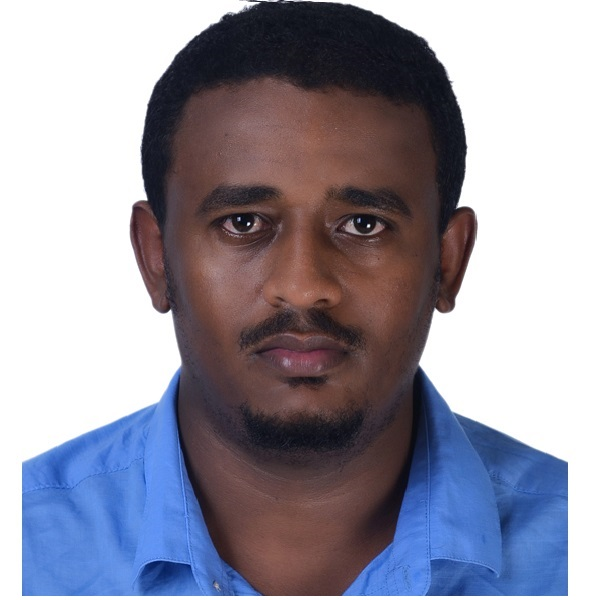
\includegraphics[width=3cm]{author.jpg}}},{}]
\end{window}
\ltwelve
Name: Ahmedin Mohammed Ahmed

Gender: Male

Date of Birth: 06~October~1985

Nationality: Ethiopia

Research Direction: Ad-hoc social networks, mobile data management, middleware design

Resume:


\twelve
2003/9~-~2006/7~~~Bahirdar~University~~~~~~~~~~~~~~~~~~~~~~~~Computer~Science~~~~~~~~~~~~~~BSc \par
2009/9~-~2011/7~~~Chongqing~University~~~~~~~~~~~~~~~~~~~~~Software~Engineering~~~~~~~~MEng \par
2011/9~-~2014/11~Dalian~University~of~Technology~~~~Computer~Sci.~and~Tech.~~~~PhD

\cleardoublepage

% Copyright Aughorization
\chapter*{}
\addcontentsline{toc}{chapter}{大连理工大学学位论文版权使用授权书}
\addcontentsline{toe}{chapter}{Dalian University of Technology Doctoral Dissertation Copyright Use Authorization}
\addcontentsline{toe}{chapter}{大连理工大学学位论文版权使用授权书}

\renewcommand{\baselinestretch}{1.61}
\vspace{-0.48cm}
\eauthorization
\authorization
\cleardoublepage
\end{document}

%%%%%%%%%%%%%%%%%% End of the file  %%%%%%%%%%%%%%%%%%%%%%%%
